\clearpage
\section{Обзор литературы}
\subsection{Истоки}
В 1949 году Дональд Хебб представил свою работу “The Organization of Behavior”, где сформулировал основное правило обучения без учителя: <<Клетки, которые активируются вместе, связаны вместе”. Более формальное описание звучит так: “Когда аксон клетки А находится достаточно близко, чтобы возбудить клетку Б, и многократно или постоянно участвует в том, чтобы её активировать, в одной или обеих клетках происходит некий процесс роста или изменение метаболизма, в результате которого эффективность А как клетки, возбуждающей активность Б увеличивается>>\footnote{Цит. по кн.: Николенко С.И <<Глубокое обучение>>, с. 95} . Это выражение можно переписать в виде формулы $\Delta w_i = \eta x_{i} y$, где $\Delta w_i$ – изменение синаптических весов нейрона i, имеющего входной сигнал $x_i$, $y$ – постсинаптический отклик (postsynaptic response),  $\eta$ -- коэффициент скорости обучения. Другими словами, правило Хебба показывает, что связь между нейронами должна усиливаться с ростом частоты совместных срабатываний. 
\par
За шесть лет до работы Дональда Хебба нейрофизиолог Уоррен Маккаллок и математик Уолтер Питтс смоделировали простейший нейрон с помощью электрической цепи. Их модель (McCulloch-Pitts neural model, MCP) представлена линейной ступенчатой функцией, которая может быть описана следующей формулой:
\begin{equation}
	y = 
	\begin{cases}
		1,& \text{если } \sum_{i}{w_i x_i} \geq \theta \text{ и } z_j = 0 \forall{j} \\
		0,& \text{в остальных случаях}
	\end{cases}
\end{equation}
где $y$ – выходное значение, $x_i$ – входное значение, $w_i$ - весовые коэффициенты, $z_j$ – тормозящий вход (inhibitory input), $\theta$ -- порог.
\par
Воспользовавшись результатами этих двух исследований, Фрэнк Розенблатт в 1958 году представил свою модель, названную перцептрон . 
\begin{figure}[h]
	\centering
	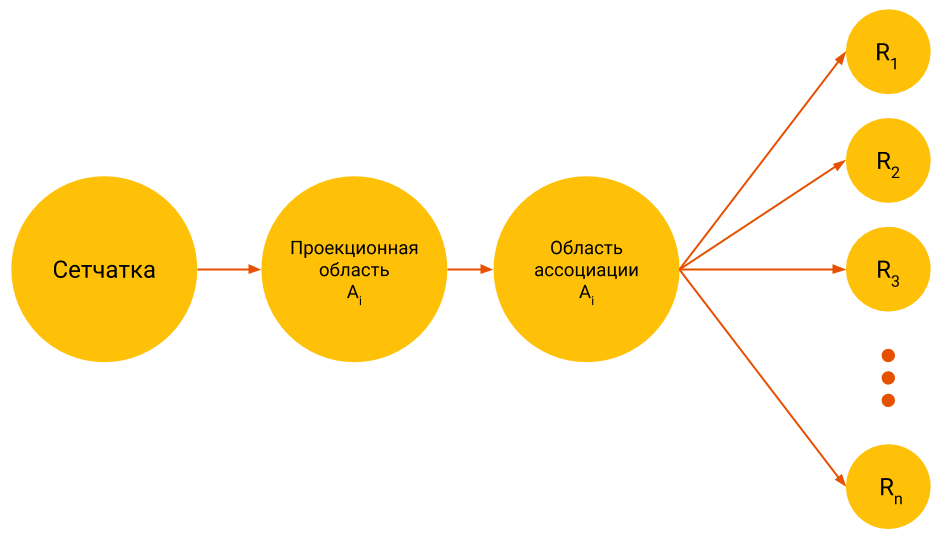
\includegraphics[width=0.8\textwidth]{perc_ros_orig}
	\caption{Оригинальная модель перцептрона Розенблатта}
	\label{hist:rosorig}
\end{figure}
\par
В работе Минского и Пейперта “Перцептроны” 1969 года были выведены ограничения возможностей одного перцептрона, а именно его линейность, то есть способность разделять только линейно разделимые множества. Очевидно, при суперпозиции нескольких линейных функций получится линейная функция, так что увеличение количество слоев сети проблему не решит. Так как уже в то время люди желали увидеть настоящий искусственный интеллект нужно было найти решение, и решением стало внесение нелинейной функции активации в модель перцептрона.
\par
В современном представлении графом вычислений один перцептрон выглядит так:
 
Где $x_1$, .., $x_n$ - входы, $w_1$, .., $w_n$ - соответствующие входам веса, h - функция активации. В дальнейшем было выделено несколько наиболее применимых функций активации: логистический сигмоид, гиперболический сигмоид, ReLU, функция Хевисайда и т.п.
\subsection{Универсальное свойство аппроксимации}
Размещая перцептроны друг с другом, мы получаем однослойную сеть, а связывая в цепочку – многослойную нейронную сеть, также известную как многослойный перцептрон (Multi-layer Perceptror, MLP). Эти конструкции из нескольких перцептронов обладали универсальным свойством аппроксимации. То есть, нейронная сеть прямого распространения способна аппроксимировать любую непрерывную функцию многих переменных с любой точностью. Это свойство было сформулировано в виде теоремы и доказано  Джорджем Цыбенко в 1989 году.
\par
Для неглубоких нейронных сетей универсальное свойство аппроксимации означает экспоненциальный рост числа нейронов, что делает использование подобных сетей затруднительным. В 2011 году Бенджио и Делалло  предположили, что было бы естественным использовать глубокие нейронные сети. 
\par
Это же умозаключение просматривается в работах Яо 1985 года об ограничениях функций неглубоких цепей. Хастад в 1986 году показал, что эти функции вычислимы в рамках булевой схемы полиномиального размера      при глубине k, но требуют экспоненциальный размер схемы при глубине, ограниченной $k-1$. Он показал это свойство главным образом применением закона Де Моргана, в котором говорится, что любые операции AND или OR могут быть переписаны как OR и AND. Опираясь на это он упростил схему, где AND и OR появляются одна за другой, переписывая один слой AND в OR и, следовательно, объединяя эту операцию со своим соседним уровнем OR. Повторяя эту процедуру, он смог представить ту же функцию с меньшим количеством слоев, но большим количеством вычислений.
\par
Возвращаясь к нейронным сетям, Бенджио и Делалло сравнивали глубокие и неглубокие сети. Они показали, что функция, которая может быть выражена $O(n)$ нейронами в сети глубины k, требует по крайней мере $O(2^{\sqrt{n}})$ и $O((n-1)^k)$ нейронов в двухслойной сети. Позже Бианчини и Скарселли обобщили эту работу на общие нейронные сети со многими важными активационными функциями, включая tanhи sigmoid.
\subsection{Метод обратного распространения ошибки}
Метод обратного распространения ошибки - это техника, позволяющая более эффективно вычислять градиент для алгоритма градиентного спуска. В сравнении с классическим алгоритмом  , который обновляет все параметры в соответствии с ошибкой, метод обратного распространения ошибки сперва вычисляет ошибку между выходным слоем и слоем, идущим перед ним. Затем к нему применяется алгоритм градиентного спуска с учетом распространенной ошибки.
\par
В 1992 году Гори и Тези изучали проблему локального минимума в методе обратного распространения ошибки. Они представили архитектуру, в которой гарантируется попадание в глобальный минимум. Для этого на нейронную сеть накладывается ряд ограничений:
\begin{enumerate}
	\item Пирамидальная архитектура. Верхние слои имеют меньше нейронов
	\item Все строки матрицы весов линейно независимы
	\item Число входных нейронов не может быть меньше числа классов данных
\end{enumerate}
Однако их подход требует, чтобы данные были линейно разделимыми. 
\par
В общем случае число локальных минимумов функции ошибки на пространстве параметров нейронной сети легко может расти экспоненциально от числа нейронов. Поэтому задача нахождения “хорошего” локального минимума нетривиальна. Для нахождения такого минимума, подобного “хорошему”, за допустимое время разрабатывались различные модификации процесса обучения и градиентного спуска соответственно, такие как:
\begin{enumerate}
	\item Обучение батчами
	\item Регуляризация
	\item Дропаут
	\item Нормализация данных
	\item Модификация Adagrad градиентного спуска
\end{enumerate}
и т.д.
\subsection{Свертка}
В 1990 году Ян Лекун совместно с группой исследователей представил архитектуру LeNet. Главной её особенностью было использование слоев свертки и подвыборки.
\begin{figure}[h]
	\centering
	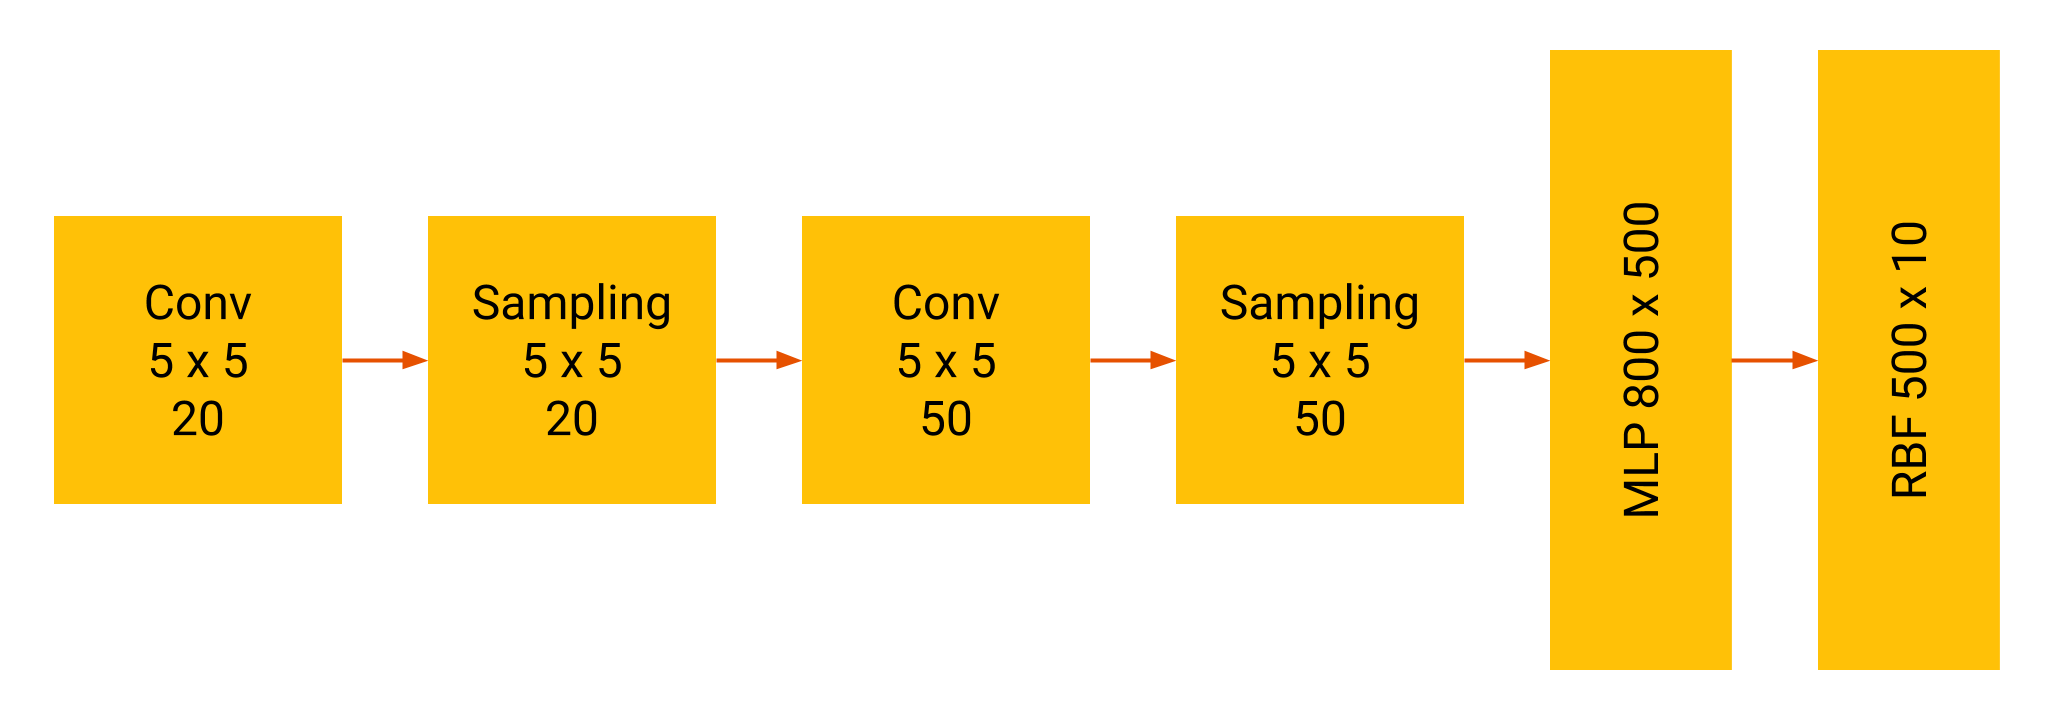
\includegraphics[width=\textwidth]{LeNet}
	\caption{Архитектура LeNet}
	\label{hist:lenet}
\end{figure}
\par
Слой свертки применяет к входным данным операцию свертки. Ее суть заключается в том, что каждый фрагмент изображения умножается на матрицу (ядро) свертки поэлементно, а результат суммируется и записывается в аналогичную позицию выходного изображения. Также сверточный слой вводит использование нелинейной активационной функции. Это позволяет нейронной сети более эффективно выделять признаки и точнее симулировать функции зрительной коры головного мозга. В качестве такой функции может использоваться ReLU (Rectified Linear Unit), которая “отсекает” отрицательную часть входных данных: $f(x) = max(0,x)$.
\begin{figure}[h]
	\centering
	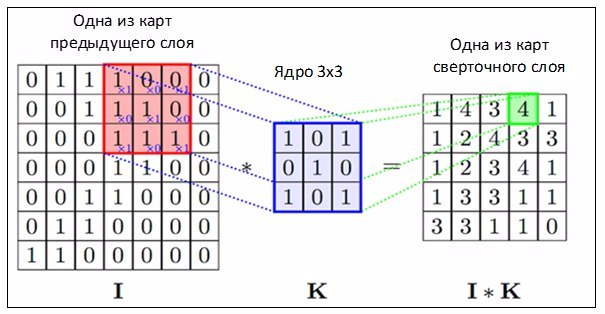
\includegraphics[width=0.8\textwidth]{conv}
	\caption{Свертка}
	\label{hist:conv}
\end{figure}
\par
Слой подвыборки выполняет более простую задачу. Он выбирает одно значение из области, в которую “смотрит”. Выбор может производиться по разным критериям: выбор максимального, подсчет среднего или выбор случайного значения. Такая операция понижает размерность данных и делает нейронную сеть инвариантной к небольшим изменениям входных данных.
\subsection{Рекуррентные нейронные сети}
В 1982 году Джон Хопфилд представил новую архитектуру сети, главной особенностью которой были двунаправленные соединения между нейронами (то есть, матрица весовых коэффициентов симметричная). Такая сеть может быть использована как ассоциативная память. Сеть Хопфилда положила начало развитию нового класса нейронных сетей, названного рекуррентными. Благодаря тому, что связи в них образуют направленную последовательность, появилась возможность обрабатывать последовательные пространственные цепочки.
\par
Другим прорывом в семействе рекуррентных нейронных сетей стало создание нового нейрона, названного долгой краткосрочной памятью (Long Short-Term Memory, LSTM),  Сеппом Хохрайтером и Юргеном Шмидхубером в 1997 году. Его целью было улучшение работы рекуррентных сетей с долгосрочными зависимостями . LSTM состоит из нескольких важных компонентов:
\begin{enumerate}
	\item Состояния - значения, использующиеся, чтобы предоставить выходную информацию
	\item Входные данные обозначены за $x$
	\item Скрытое состояние - значения предыдущих скрытых слоев. Обозначено за $h$
	\item Входное состояние - линейная комбинация скрытого состояния и входа в текущий момент времени. Обозначено за $i$. $i^t = \sigma(W_{ix} x^t + W_{ih} h^{t-1})$
	\item Внутреннее состояние - служит “памятью”, обозначено за $m$
	\item Вентили - значения, определяющие потоки данных
	\item Входной вентиль определяет, войдет ли входное состояние во внутреннее. $g^t=\sigma (W_{gi} i^t)$.
	\item Вентиль забывания определяет, забывает ли внутреннее состояние предыдущее внутреннее состояние. $f^t=\sigma(W_{fi} i^t)$
	\item Выходной вентиль определяет, передает ли внутреннее состояние свое значение выходу и скрытому состоянию в следующий момент времени. $o^t=\sigma(W_{oi} i^t)$
	\item С учетом приведенных выше формул можем получить математическую модель LSTM-ячейки: 
		\begin{equation}
			\begin{gathered}
				m^t = g^t \odot i^t + f^t m^{t-1},\\
				h^t = o^t \odot m^t
			\end{gathered}
		\end{equation}
\end{enumerate}

